\documentclass[a4paper,5pt]{amsbook}
%%%%%%%%%%%%%%%%%%%%%%%%%%%%%%%%%%%%%%%%%%%%%%%%%%%%%%%%%%%%%%%%%%%%%

\usepackage{booktabs}
\usepackage{graphicx}
\usepackage{multicol}
\usepackage{textcomp}
\usepackage{systeme}
\usepackage{amssymb}
\usepackage[]{amsmath}
\usepackage{subcaption}
\usepackage[inline]{enumitem}

%%%%%%%%%%%%%%%%%%%%%%%%%%%%%%%%%%%%%%%%%%%%%%%%%%%%%%%%%%%%%%

\newcommand{\sen}{\,\mbox{sen}\,}
\newcommand{\tg}{\,\mbox{tg}\,}
\newcommand{\cosec}{\,\mbox{cosec}\,}
\newcommand{\cotg}{\,\mbox{cotg}\,}
\newcommand{\tr}{\,\mbox{tr}\,}
\newcommand{\ds}{\displaystyle}

%%%%%%%%%%%%%%%%%%%%%%%%%%%%%%%%%%%%%%%%%%%%%%%%%%%%%%%%%%%%%%%%%%%%%%%%

\setlength{\textwidth}{16cm} \setlength{\topmargin}{-2cm}
\setlength{\textheight}{25cm}
\setlength{\leftmargin}{1.2cm} \setlength{\rightmargin}{1.2cm}
\setlength{\oddsidemargin}{0cm}\setlength{\evensidemargin}{0cm}

%%%%%%%%%%%%%%%%%%%%%%%%%%%%%%%%%%%%%%%%%%%%%%%%%%%%%%%%%%%%%%%%%%%%%%%%

% \renewcommand{\baselinestretch}{1.6}
% \renewcommand{\thefootnote}{\fnsymbol{footnote}}
% \renewcommand{\theequation}{\thesection.\arabic{equation}}
% \setlength{\voffset}{-50pt}
% \numberwithin{equation}{chapter}

%%%%%%%%%%%%%%%%%%%%%%%%%%%%%%%%%%%%%%%%%%%%%%%%%%%%%%%%%%%%%%%%%%%%%%%

\begin{document}
\thispagestyle{empty}
\pagestyle{empty}
\begin{minipage}[h]{0.14\textwidth}
	
\includegraphics[scale=0.24]{../../ufgd.png}
\end{minipage}
\begin{minipage}[h]{\textwidth}
\begin{tabular}{c}
{{\bf UNIVERSIDADE FEDERAL DA GRANDE DOURADOS}}\\
{{\bf \'{A}lgebra Linear e Geometria Anal\'{\i}tica --- Lista 4}}\\
{{\bf Prof.\ Adriano Barbosa}}\\
\end{tabular}
\vspace{-0.45cm}
%
\end{minipage}

%------------------------

%%%%%%%%%%%%%%%%%%%%%%%%%%%%%%%%   formulario  inicio  %%%%%%%%%%%%%%%%%%%%%%%%%%%%%%%%
\begin{enumerate}
	\vspace{0.5cm}
	\item Encontre o segmento orientado com ponto inicial $P = (-1, 3, -5)$ tal
		que
		\begin{enumerate}
			\item Tem a mesma dire\c{c}\~ao e sentido que o vetor $v = (6, 7, -3)$
			\item Tem a mesma dire\c{c}\~ao mas sentido oposto ao de $v = (6, 7, -3)$
		\end{enumerate}

	\vspace{0.5cm}
	\item Sejam $u = (-3, 1, 2)$, $v = (4, 0, -8)$ e $w = (6, -1, -4)$. Calcule

		\begin{enumerate*}
			\item $v-w$
			\hspace{0.5cm}
			\hspace{0.5cm}
			\item $6u+2v$
			\hspace{0.5cm}
			\hspace{0.5cm}
			\item $-3(v-8w)$
			\hspace{0.5cm}
			\hspace{0.5cm}
			\item $(2u-7w)-(8v+u)$
		\end{enumerate*}

	\vspace{0.5cm}
	\item Dados tr\^es pontos $A$, $B$ e $C$, represente graficamente os
		segmentos orientados

	\begin{minipage}{0.4\textwidth}
		\begin{enumerate}
			\item $BA + 2 BC$
			\vspace{0.2cm}
			\item $2 CA + 2 BA$
			\vspace{0.2cm}
			\item $3 AB - 2 BC$
			\vspace{0.2cm}
			\item $\ds\frac{1}{2} AB - 2 CB$
		\end{enumerate}
	\end{minipage}
	\begin{minipage}{0.4\textwidth}
		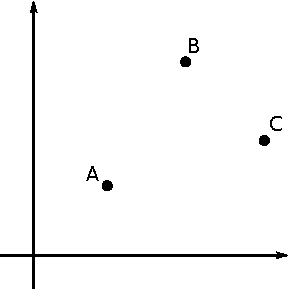
\includegraphics[scale=0.6]{lista-04-fig02.pdf}
	\end{minipage}
 
	\vspace{0.5cm}
	\item \'E poss\'{\i}vel encontrar escalares $a, b$ e $c$ tais que
		$a(-2,9,6)+b(2,1,1)+c(0,3,1)=(0,0,0)$?

	\vspace{0.5cm}
	\item Calcule as coordenadas dos vetores $u$, $v$, $u+v$ e $u-v$ abaixo
		\begin{figure}[h]
			\centering
			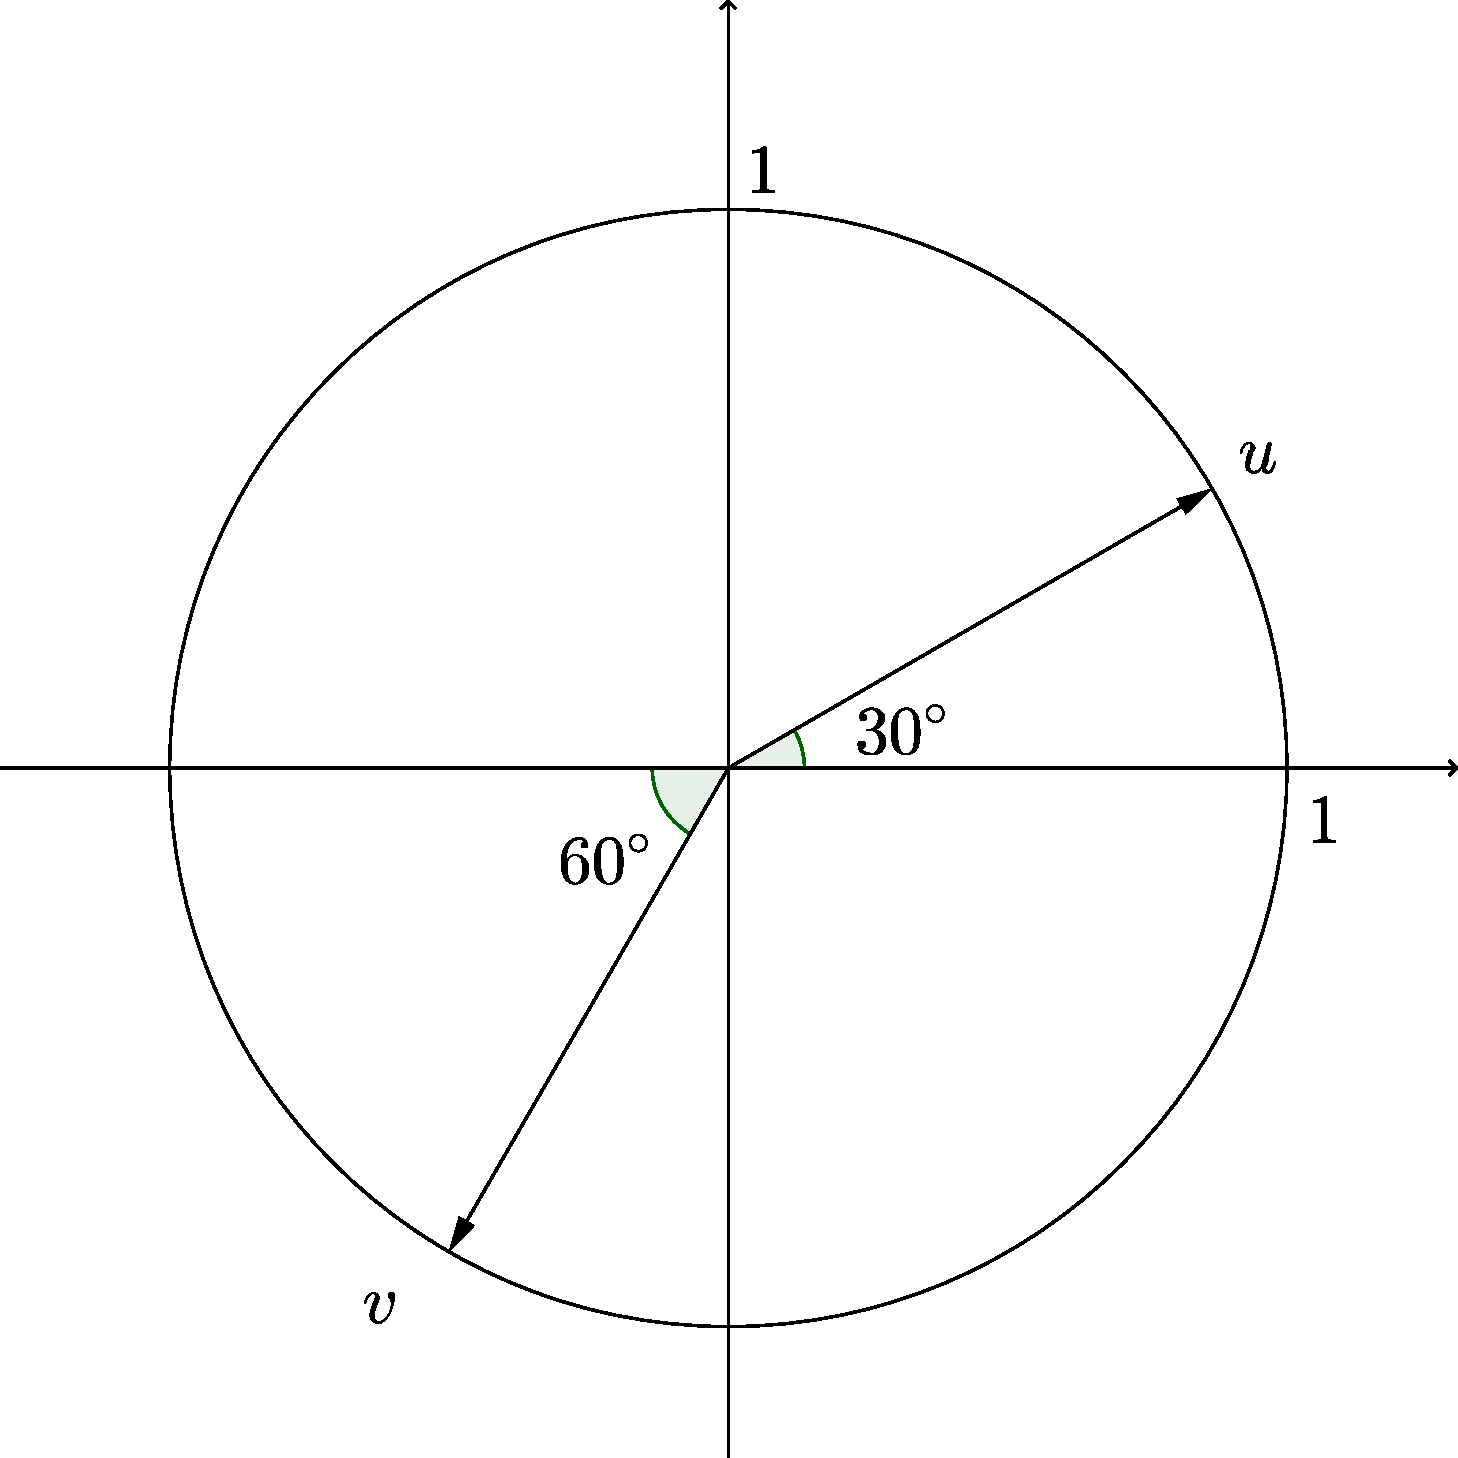
\includegraphics[width=5cm]{lista-04-fig01.pdf}
		\end{figure}

	\vspace{0.5cm}
	\item Sejam $u=(2,-2,3)$, $v=(1,-3,4)$ e $2=(3,6,-4)$. Calcule

		\begin{enumerate*}
			\item $\|u+v\|$
			\hspace{0.5cm}
			\hspace{0.5cm}
			\item $\|3u-5v+w\|$
			\hspace{0.5cm}
			\hspace{0.5cm}
			\item $\ds\frac{1}{\|w\|}w$
		\end{enumerate*}

	\vspace{0.5cm}
	\item Sejam $p_0=(x_0,y_0,z_0)$ e $p=(x,y,z)$. Descreva o conjunto de
		pontos $(x,y,z)$ para os quais $\|p-p_0\|=1$.

	\vspace{0.5cm}
    \item Verifique geometricamente que $\|u+v\|\le\|u\|+\|v\|$, quaisquer que
        sejam os vetores $u$ e $v$.

	\vspace{0.5cm}
	\item Decida se as afirma\c{c}\~oes s\~ao verdadeiras ou falsas:
	\begin{enumerate}
		% \item Se $u = v$, ent\~ao $\|u\| = \|v\|$.
		\item Se $\|u\| = \|v\|$, ent\~ao $u = v$.
		\item Se $u$ \'e paralelo a $v$, ent\~ao $u = v$.
		\item Se $u = v$, ent\~ao $u$ \'e paralelo a $v$.
		\item Se $w = u + v$, ent\~ao $\|w\| = \|u\| + \|v\|$.
		\item $\|w\| = \|u\| + \|v\|$, ent\~ao $u$, $v$ e $w$ s\~ao paralelos.
		% \item $\|5v\| = \|-5v\| = 5\|v\|$.
		% \item Os vetores $3v$ e $-4v$ s\~ao paralelos e de mesmo sentido.
		\item Se $u$ \'e paralelo a $v$, $\|u\| = 2$ e $\|v\| = 4$, ent\~ao $v = 2u$ ou $v = -2u$.
	\end{enumerate}

	\vspace{0.5cm}
	\item Encontre $\langle u, v \rangle$ e o \^angulo entre $u$ e $v$:

		\begin{enumerate*}
			\item $u=(2,3)$ e $v=(5, -7)$
			\hspace{0.5cm}
			\hspace{0.5cm}
			\item $u=(-2,2,3)$ e $v=(1,7,-4)$
		\end{enumerate*}

	\vspace{0.5cm}
	\item Mostre que os vetores $u=(a,b)$ e $v=(-b,a)$ s\~ao ortogonais. Encontre
		dois vetores ortogonais a $u=(2,-3)$. 

	\vspace{0.5cm}
	\item Dados $u=(3,2,-1)$, $v=(0,2,-3)$ e $w=(2,6,7)$. Calcule

		\begin{enumerate*}
			\item $v\times w$
			\hspace{0.5cm}
			\hspace{0.5cm}
			\item $u \times (v-2w)$
			\hspace{0.5cm}
			\hspace{0.5cm}
			\item $(u \times v) \times (v \times w)$
		\end{enumerate*}

	\vspace{0.5cm}
	\item Encontre a \'area do tri\^angulo de v\'ertices $(2,6,-1)$, $(1,1,1)$ e $(4,6,2)$.
	
	\vspace{0.5cm}
	\item Encontre um vetor ortogonal ao vetor $u=(2,-3,5)$.

	\vspace{0.5cm}
	\item Suponha $\langle u, v \times w \rangle = 3$. Encontre

		\begin{enumerate*}
			\item $\langle u, w \times v \rangle$
			\hspace{0.5cm}
			\hspace{0.5cm}
			\item $\langle v \times w, u \rangle$
			\hspace{0.5cm}
			\hspace{0.5cm}
			\item $\langle w, u \times v \rangle$
			\hspace{0.5cm}
			\hspace{0.5cm}
			\item $\langle v, u \times w \rangle$
		\end{enumerate*}

	\vspace{0.5cm}
	\item Determine se os vetores $u$, $v$ e $w$ est\~ao num mesmo plano:
		\begin{enumerate}
			\item $u=(-1,-2,1)$, $v=(3, 0, -2)$ e $w = (5,-4,0)$
			\item $u=(4,-8,1)$, $v=(2,1,-2)$ e $w=(3,-4,12)$
			\item $u=(1,2)$, $v=(3,4)$ e $w=(5,6)$
		\end{enumerate}
\end{enumerate}

\end{document}
